
\chapter{Discussion}
\label{cha:discussion}

\section{Observation}
Difference between levels that are easy for humans and computers.

\subsection{Patterns}
Some levels contains an overall pattern which humans will easily spot while the computer will have a hard time solving the puzzle. A pattern could be where the player has to push the boxes in chain reaction.

An example of this is shown in \ref{fig:level7}. A human player will quite fast spot that the level is build up by a circle of boxes only moveable by moving one of the bottom boxes to the midle and then by moving the box above its startposition one square down. Following this direction around the circle all the boxes can be put onto a goal square. The computer will have to try alot of moves before finding the correct pattern.

\begin{figure}[htp]
	\centering
	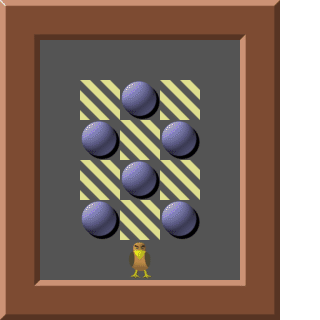
\includegraphics[scale=0.5]{level7}
	\caption{Level 7 - a level with a pattern easy to spot for a human}
	\label{fig:level7}
\end{figure}

\subsection{Deadlock detection}
Solving Sokobano puzzles is much about avoiding deadlocked states. As
it can be hard to describe when a state contains a deadlock and hard
to check if it has one in a very short time, human players might be
better at spotting these states. Though the computer would ``just''
need a better deadlock detection than what we have been able to come
up with.

\section{Improvements}
\subsection{More deadlock detection}
To improve the algorithm, better deadlock detections must be
created. The first to implement would be heuristics that detect the
states in figure \ref{fig:missingdeadlocks}.

First of all it should not be allowed to put two boxes into the same
narrow corridor as you cannot get in between the boxes thus making the
boxes deadlock. (The left image in figure \ref{fig:missingdeadlocks}.)
One way of solving this could be to make the corridor a one box only
zone and lock it as soon as a box is inside it.

Furthermore a deadlock detector that is able to check if a room with
only one entrance is getting blocked, must be created. (The right
image). There are many aspects in this: first of all how do you find
areas with only one entrance? And how do you decide whther the
entrance is blocked? And how do you do this without making the
algorithm very slow?

\begin{figure}[htp]
  \centering
  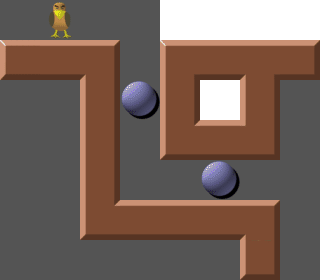
\includegraphics[totalheight=0.2\textheight]{narrow}
  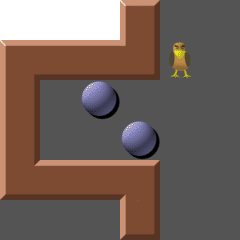
\includegraphics[totalheight=0.2\textheight]{blockedentrance}
  \caption{Deadlocks not found by our heuristics}
  \label{fig:missingdeadlocks}
\end{figure}

\subsection{A different planning method}
To improve the algorithm a different planning method could be used. We will try to argue if \textit{POP planning} and \textit{Regression planning} could improve the planning algorithm further.
\subsubsection{POP planning}
Using Partial order planning to solve planning problems require the problem to be dividable into independent subproblems. In most Sokoban problems this is not possible as the moving one box influences the solution for the other boxes. Furthermore the a box almost always have to be moved in order to get another box in to a goal.

\subsubsection{Regression planning}
Regression planning might work better than progression planning as the puzzles might be created bearing in mind that the solution should be hard to find from the beginning. Especially if the branches a lot in the early states an less in the later a regression planner might work great. At the same time it might work quite bad as well, especially on big but easy maps, as they might be created bearing in mind that the level should be easy to solve using progression planning.

Many levels contain a goal area where all boxes have to get into. These are easier to solve using progression planning as it does not matter which box goes to which goal square. Using regression planning on these maps might be hard as the algorithm would have to find out which box to place at its startposition first.

\section{Other variants of Sokoban}
There exists a number of variants of Sokoban-like games. Some of these variants might be solvable by the planner by making small modifications to the planner while others might be almost imposible to solve.

\begin{description}
\item[Colored boxes] One variant is to play Sokoban with colored boxes and goals. The objective would then be to get a box with a given color put on a goal of the same color. Our planner would probably be able to solve the problem if the distance heuristics measured the distance between boxes and goals of the same color instead of the distance to all/the nearest goal(s).
\item[Several Pushers] Another variant might let the there be more than one player/pusher. In order to solve the puzzles the players would have to cooperate. Our implementation does not allow more than one player, but even if it had it would be hard to find a solution as the number of possible actions in each state would rise quite fast with the number of players. The number of searched states would then grow bigger even faster and thereby make it harder to find a solution. The heuristics would have a hard time figuring out which states are good as the order in which the players would be moved would make lots of parallel paths.
\item[Push rows of boxes] If it was allowed to push rows of boxes this action would have to be implemented. But after having done this the levels might still be solvable by the planner we have created. As long as the heuristics are good at estimating the performance more actions will only have a small influence on the solution. More actions would mean that more states would be discovered, but only one of these states would be placed in the top of the queue. As opposed to the \textit{Several Pushers} variant the paths of the new actions would not create alot of parallel paths.
\item[Doors] The last variant we could think of is a variant having doors which would only open when a box is placed on a button or only letting the player pass through without a box. Doors only opening when a box is placed on a button would require the planner being able to solve the goal of getting a box on the button before trying to plan its way through the door. This would require a completely new planner. Doors only allowing the player to pass could easily be implemented using the method used by the \textit{Corner Heuristic} (See section \ref{sec:cornerheur}) marking the door an illegal square. Such a Sokoban map would probably be solvable by the planner.
\end{description}
